\documentclass[11pt]{ctexart}

\usepackage[margin=1in]{geometry}
\usepackage{amsmath, amssymb}
\usepackage{booktabs}
\usepackage{graphicx}
\usepackage{float}
\usepackage{hyperref}
\usepackage{algorithm2e}
\usepackage{fontspec}
\usepackage{xcolor}
\usepackage{caption}
\usepackage{subcaption}

\setmainfont{TeX Gyre Pagella}
\setCJKmainfont{Noto Serif CJK SC}
\setmonofont{DejaVu Sans Mono}
\graphicspath{{../../../result/}{../assets/}}

\hypersetup{
  colorlinks=true,
  linkcolor=blue!55!black,
  urlcolor=blue!55!black,
  citecolor=blue!55!black
}

\SetAlgorithmName{算法}{算法}{算法列表}
\DontPrintSemicolon
\SetKwInput{KwInput}{输入}
\SetKwInput{KwOutput}{输出}

\setcounter{secnumdepth}{3}
\renewcommand{\thesubsection}{\arabic{subsection}}
\renewcommand{\thesubsubsection}{\thesubsection.\arabic{subsubsection}}

\newcommand{\problem}[1]{\subsection{#1}}
\newcommand{\blocktitle}[1]{\subsubsection{#1}}
\newcommand{\plainblocktitle}[1]{\paragraph{#1}\mbox{}\\}

\title{Homework 14 Report\\\large 原生 \LaTeX{} 试验版}
\author{姜玥晟}
\date{2026-06-10}

\begin{document}
\maketitle

\begin{figure}[H]
  \centering
  
\includegraphics[width=0.18\linewidth]{profile.jpg}
\end{figure}

\begin{table}[H]
  \centering
  \begin{tabular}{lp{0.68\linewidth}}
    \toprule
    项目 & 内容 \\
    \midrule
    源题编号 & Homework 14 \\
    学生姓名 & 姜玥晟 \\
    报告主题 & Ising 模型的 Monte Carlo 模拟 \\
    实验环境 & Python 3.13.5、numpy 2.3.3、matplotlib 3.10.7、scipy 1.16.2 \\
    统一单位 & $J=1,\ k_B=1,\ h=0$ \\
    随机种子 & 20260610 \\
    \bottomrule
  \end{tabular}
\end{table}

\newpage

\section*{I. 一维 Ising 模型的 Metropolis 模拟}

\problem{Problem 1(a)：有序初态的平衡时间}

\blocktitle{待求问题}
取 $N=20,\ T=1.0$，初态为所有自旋向上。计算每个 MC sweep 后的能量，并估计系统达到平衡所需的步数。

\blocktitle{解决方式}
一维周期边界链的能量为
\[
  E=-J\sum_{i=1}^{N}s_i s_{i+1},\qquad s_i=\pm 1.
\]
单自旋翻转的能量变化为
\[
  \Delta E=2J s_i(s_{i-1}+s_{i+1}).
\]
若 $\Delta E\le 0$ 则接受，否则以 $\exp(-\Delta E/T)$ 的概率接受。

\begin{algorithm}[H]
  \caption{一维 Metropolis 更新}
  \KwInput{$N,T,n_{\mathrm{sweeps}}$ 和初始构型}
  \KwOutput{逐 sweep 的 $E,M$ 和接受率}
  初始化自旋、能量 $E$ 和磁化 $M$\;
  \For{$s=1$ \KwTo $n_{\mathrm{sweeps}}$}{
    $a\leftarrow 0$\;
    \For{$r=1$ \KwTo $N$}{
      均匀随机选择格点 $i$\;
      计算 $\Delta E=2J s_i(s_{i-1}+s_{i+1})$\;
      \If{$\Delta E\le 0$ 或 $u<\exp(-\Delta E/T)$}{
        翻转 $s_i$，增量更新 $E,M$，并令 $a\leftarrow a+1$\;
      }
    }
    记录 $E,M,a/N$\;
  }
\end{algorithm}

\blocktitle{问题答案}
题目给出的理论能量公式在 $N=20,T=1$ 时给出
\[
  \langle E\rangle=-N\tanh(1/T)=-20\tanh(1)=-15.232.
\]
全向上初态的估计平衡时间约为 59 个 sweep；后 500 个 sweep 给出
\[
  \langle E\rangle=-15.216,\qquad
  \langle M\rangle=0.804,\qquad
  \langle |M|\rangle=9.572,\qquad
  A=0.245.
\]
这里 $\langle M\rangle$ 是带符号磁化，长时间平衡极限下应因 $M\leftrightarrow -M$ 对称而趋近 0；$\langle |M|\rangle$ 不会被正负翻转抵消，更能反映有限链的有序程度。

\begin{figure}[H]
  \centering
  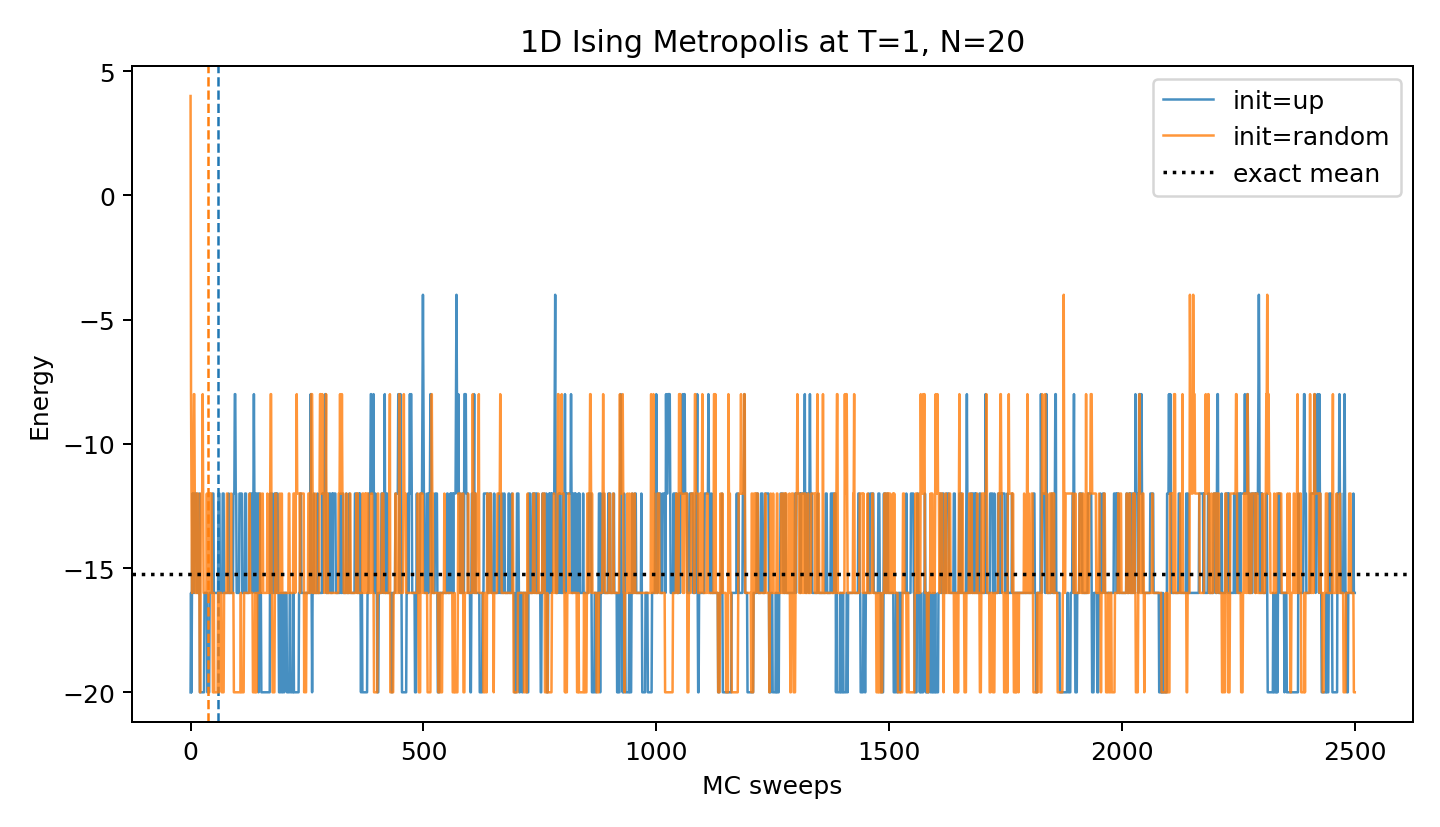
\includegraphics[width=0.72\linewidth]{problem1_equilibration.png}
  \caption{一维 Metropolis 在 $T=1$ 时的能量弛豫。}
\end{figure}

\blocktitle{理解}
低温下升能翻转被压制，全向上初态需要由热涨落产生畴壁对后才能接近平衡能量；因此弛豫曲线有明显的离散跳变和较强相关。59 个 sweep 是基于滑动平均判据的有限轨迹估计，不是唯一的解析弛豫时间。

\problem{Problem 1(b)--(d)：随机初态、温度扫描与接受率}

\blocktitle{待求问题}
随机初始化自旋并估计平衡时间；在 $T=0.5$ 到 $5.0$ 的范围内计算平均能量、磁化和接受率，并与精确能量公式比较。

\blocktitle{解决方式}
每个温度点运行 1300 个 sweep，舍去前 100 个 sweep。零场下 signed magnetization 受 $M\leftrightarrow -M$ 对称性影响，因此同时统计 $\langle |M|\rangle$。比较基准为
\[
  \langle E\rangle=-N\tanh(1/T).
\]

\blocktitle{问题答案}
随机初态的估计平衡时间约为 37 个 sweep；后 500 个 sweep 给出
\[
  \langle E\rangle=-14.888,\qquad
  \langle M\rangle=0.128,\qquad
  \langle |M|\rangle=9.280,\qquad
  A=0.258.
\]

\begin{table}[H]
  \centering
  \caption{随机初态的一维温度扫描。}
  \begin{tabular}{rrrrrr}
    \toprule
    $T$ & $\langle E\rangle$ & 精确值 & $\langle M\rangle$ & $\langle |M|\rangle$ & 接受率 \\
    \midrule
    0.5 & -19.983 & -19.281 & 19.987 & 19.99 & 0.001 \\
    1.0 & -15.287 & -15.232 & 2.280 & 10.12 & 0.232 \\
    1.5 & -11.767 & -11.656 & 0.825 & 6.88 & 0.416 \\
    2.0 & -9.200 & -9.242 & 0.232 & 5.64 & 0.545 \\
    2.5 & -7.690 & -7.599 & 0.340 & 5.41 & 0.618 \\
    3.0 & -6.547 & -6.430 & 0.338 & 5.16 & 0.675 \\
    3.5 & -5.480 & -5.564 & -0.098 & 4.73 & 0.727 \\
    4.0 & -4.903 & -4.898 & -0.523 & 4.25 & 0.754 \\
    4.5 & -4.393 & -4.373 & -0.045 & 4.28 & 0.781 \\
    5.0 & -3.657 & -3.948 & 0.198 & 4.24 & 0.807 \\
    \bottomrule
  \end{tabular}
\end{table}

\begin{figure}[H]
  \centering
  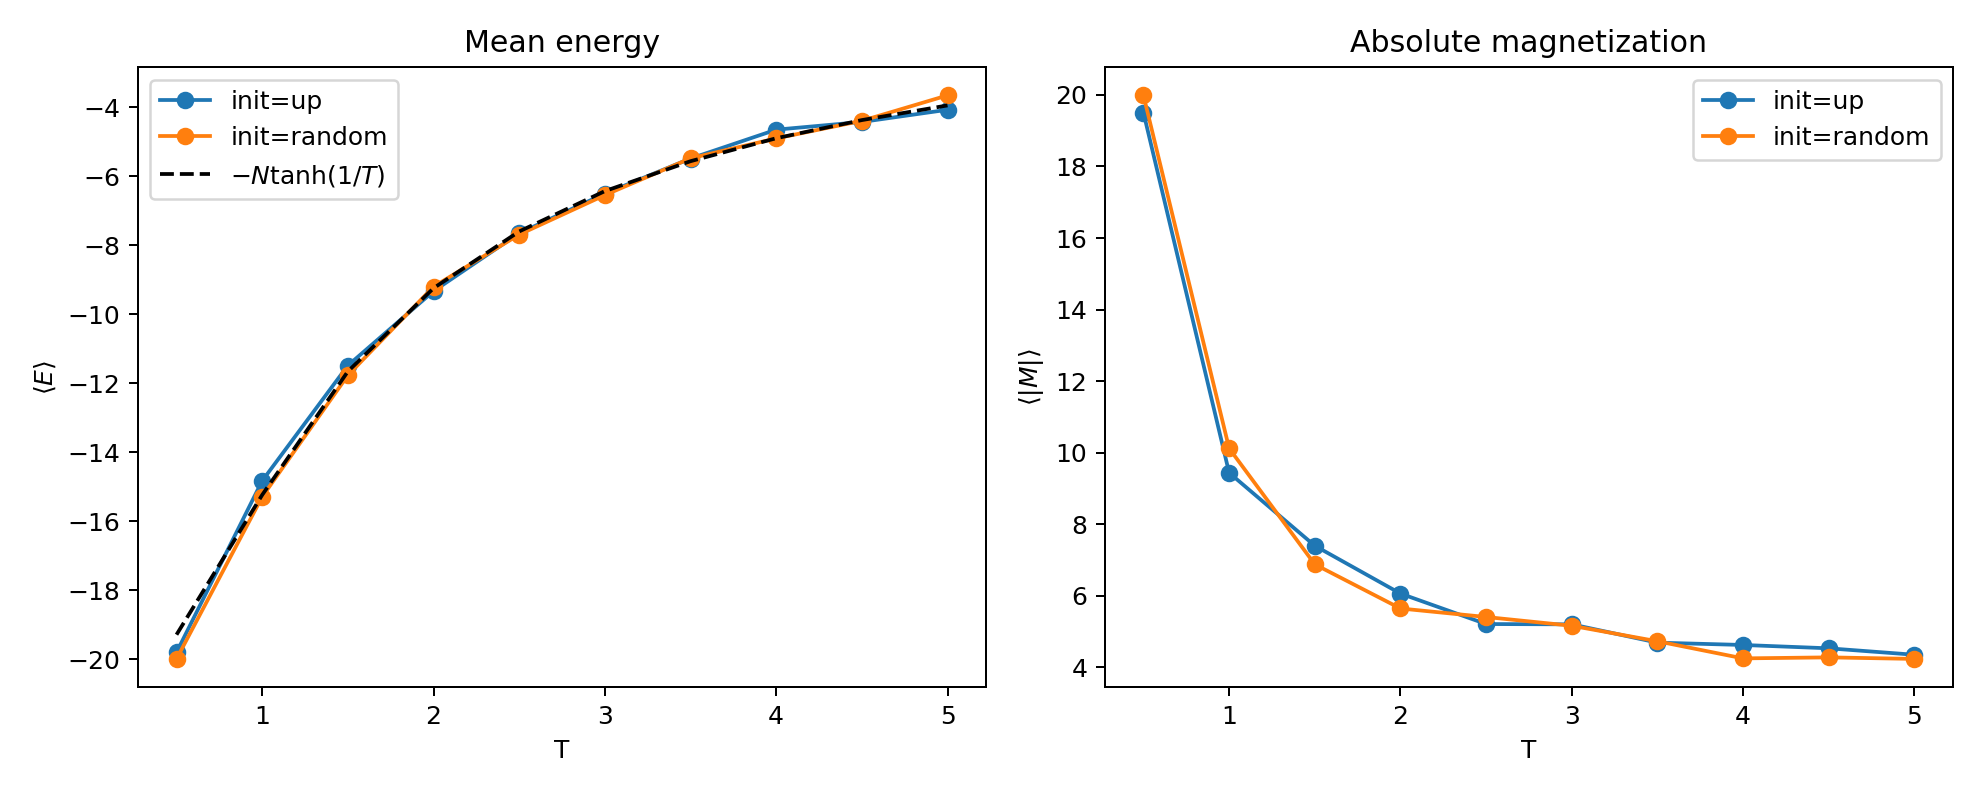
\includegraphics[width=0.80\linewidth]{problem1_temperature_scan.png}
  \caption{一维链的温度扫描。}
\end{figure}

\blocktitle{理解}
能量随温度升高而上升，接受率也随温度升高而增大。低温时算法更容易慢混合，因为大多数升能翻转概率很小。零外场下充分长时间平均的 signed $\langle M\rangle$ 应趋近 0；表中低温点的非零 $\langle M\rangle$ 说明有限时间轨迹可能仍保留初态或随机涨落造成的磁化方向记忆。因此题目问 $\langle M\rangle$ 是否依赖初态时，答案是：有限运行中会依赖，充分平衡的零场系综平均不应依赖，并趋近 0。

\section*{II. 一维 Ising 模型的 demon 算法}

\problem{Problem 2(a)--(d)：微正则 demon 模拟}

\blocktitle{待求问题}
在 $N=100,\ J=1,\ h=0$ 的一维链中实现 demon 算法，给出 $E_{\mathrm{tot}}=-20$ 的平衡量，并对 $E_{\mathrm{tot}}=-40,-60,-80$ 计算温度和能量。

\blocktitle{解决方式}
初态全向上时 $E_s=-100$。给定总能量 $E_{\mathrm{tot}}$ 后，demon 初能量为
\[
  E_d=E_{\mathrm{tot}}-E_s.
\]
接受规则为 $\Delta E\le E_d$，接受后更新
\[
  E_s\leftarrow E_s+\Delta E,\qquad
  E_d\leftarrow E_d-\Delta E.
\]

\begin{algorithm}[H]
  \caption{一维 demon 更新}
  \KwInput{$N,E_{\mathrm{tot}},n_{\mathrm{sweeps}}$}
  \KwOutput{$E_s,E_d,M,M^2$ 的时间序列}
  全向上初始化，并设置 $E_d=E_{\mathrm{tot}}-E_s$\;
  \For{每个 sweep}{
    \For{$r=1$ \KwTo $N$}{
      随机选择格点 $i$ 并计算翻转能量差 $\Delta E$\;
      \If{$\Delta E\le E_d$}{
        接受翻转；$E_s\leftarrow E_s+\Delta E$；$E_d\leftarrow E_d-\Delta E$\;
      }
    }
    记录 $E_s,E_d,M,M^2$\;
  }
\end{algorithm}

温度由离散 demon 能量关系确定：
\[
  \frac{k_BT}{J}=\frac{4}{\ln(1+4J/\langle E_d\rangle)}.
\]

\blocktitle{问题答案}
$E_{\mathrm{tot}}=-20$ 时，运行平均约在 60 sweep 后稳定，得到
\[
  \langle E_d\rangle=2.142,\quad
  \langle E_s\rangle=-22.142,\quad
  T=3.797,\quad
  \langle M^2\rangle=152.574.
\]

\begin{table}[H]
  \centering
  \caption{不同总能量下的 demon 温度与系统能量。}
  \begin{tabular}{rrrrrr}
    \toprule
    $E_{\mathrm{tot}}$ & $\langle E_d\rangle$ & $T$ & $\langle E\rangle/N$ & 精确 $E/N$ & $\langle M^2\rangle/N^2$ \\
    \midrule
    -40 & 0.705 & 2.107 & -0.407 & -0.442 & 0.0219 \\
    -60 & 0.238 & 1.389 & -0.602 & -0.617 & 0.0356 \\
    -80 & 0.039 & 0.862 & -0.800 & -0.821 & 0.0710 \\
    \bottomrule
  \end{tabular}
\end{table}

\begin{figure}[H]
  \centering
  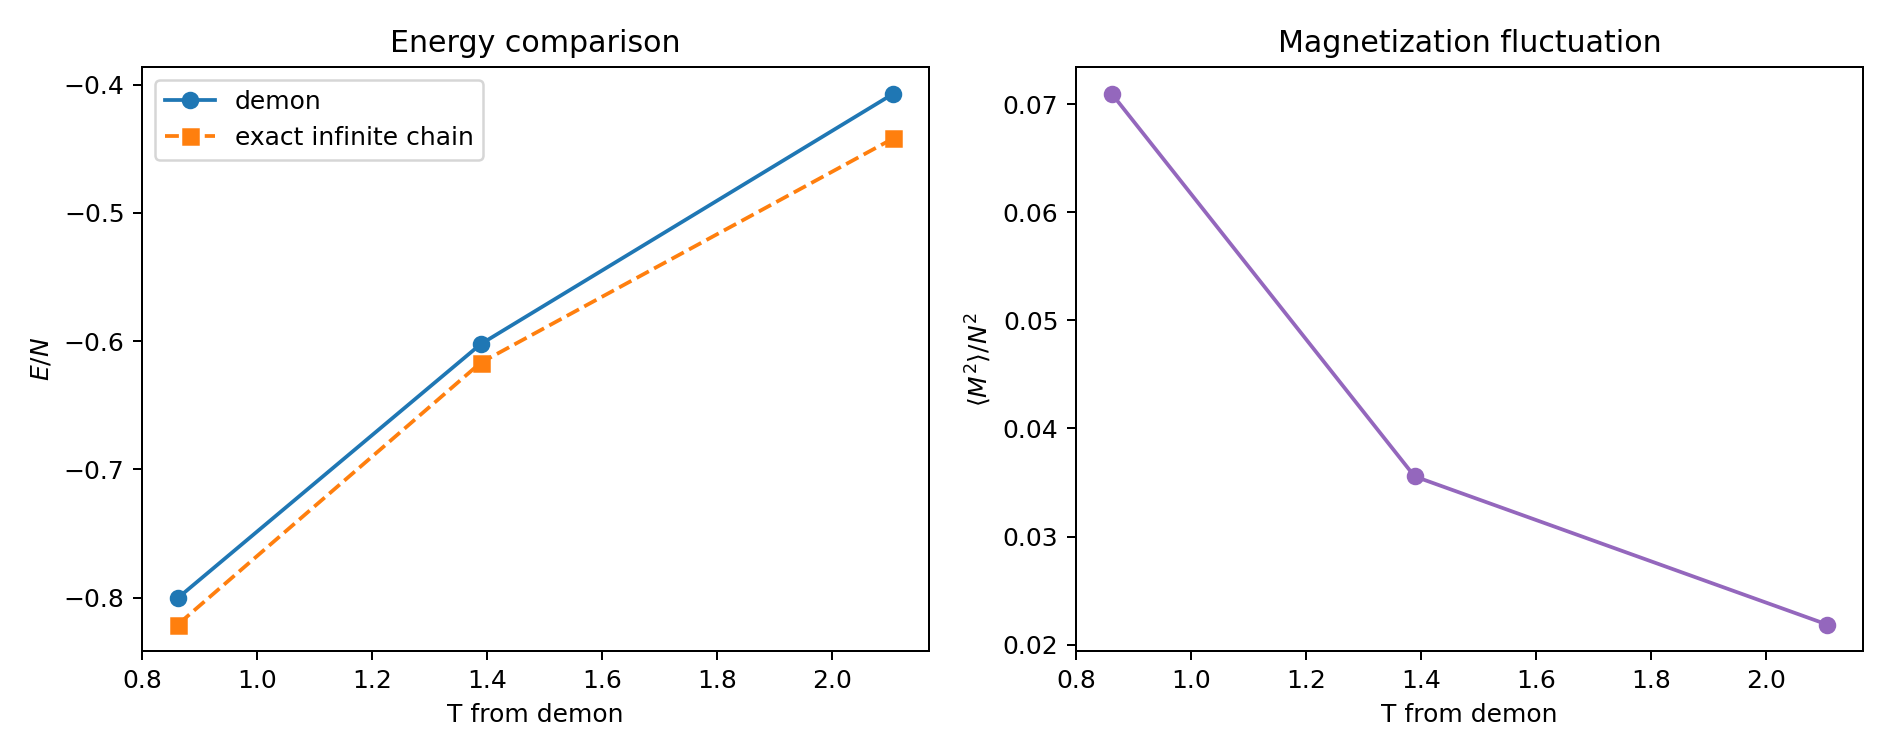
\includegraphics[width=0.82\linewidth]{problem2_demon_cases.png}
  \caption{demon 算法的能量比较与磁化平方。}
\end{figure}

\blocktitle{理解}
总能量越负，demon 可用能量越少，反推出的温度越低；低温下畴更长，因而 $\langle M^2\rangle/N^2$ 较大。

\section*{III. 二维正方格 Ising 模型}

\problem{Problem 3(a)--(b)：$T=2$ 与 $T=4$ 的弛豫}

\blocktitle{待求问题}
在 $L=30$ 的二维正方格上，使用周期边界和单自旋翻转动力学，分别考察 $T=2$ 与 $T=4$ 的能量、磁化轨迹和末态图样。

\blocktitle{解决方式}
二维能量为
\[
  E=-J\sum_{\langle i,j\rangle}s_i s_j.
\]
红黑子格更新把一个 sweep 拆成两个互不相邻的子格更新，使图像和表格扫描更容易稳定复现。

\begin{algorithm}[H]
  \caption{二维红黑子格 Metropolis sweep}
  \KwInput{$L,T$ 和当前构型}
  \KwOutput{更新后的构型以及 $E/N,|M|/N$}
  \For{parity $\in\{\mathrm{red},\mathrm{black}\}$}{
    对当前子格计算所有最近邻和 $\sum_{\mathrm{nn}}s_j$\;
    计算 $\Delta E=2J s_i\sum_{\mathrm{nn}}s_j$\;
    对子格内所有格点应用 Metropolis 接受准则\;
    同步翻转被接受的格点\;
  }
  记录 $E/N$ 与 $|M|/N$\;
\end{algorithm}

\blocktitle{问题答案}
$T=2<T_c$ 时估计热化时间约 38 sweep，后段 $E/N=-1.734$，$\langle |m|\rangle=0.908$；$T=4>T_c$ 时后段 $E/N=-0.557$，$\langle |m|\rangle=0.052$。

\begin{figure}[H]
  \centering
  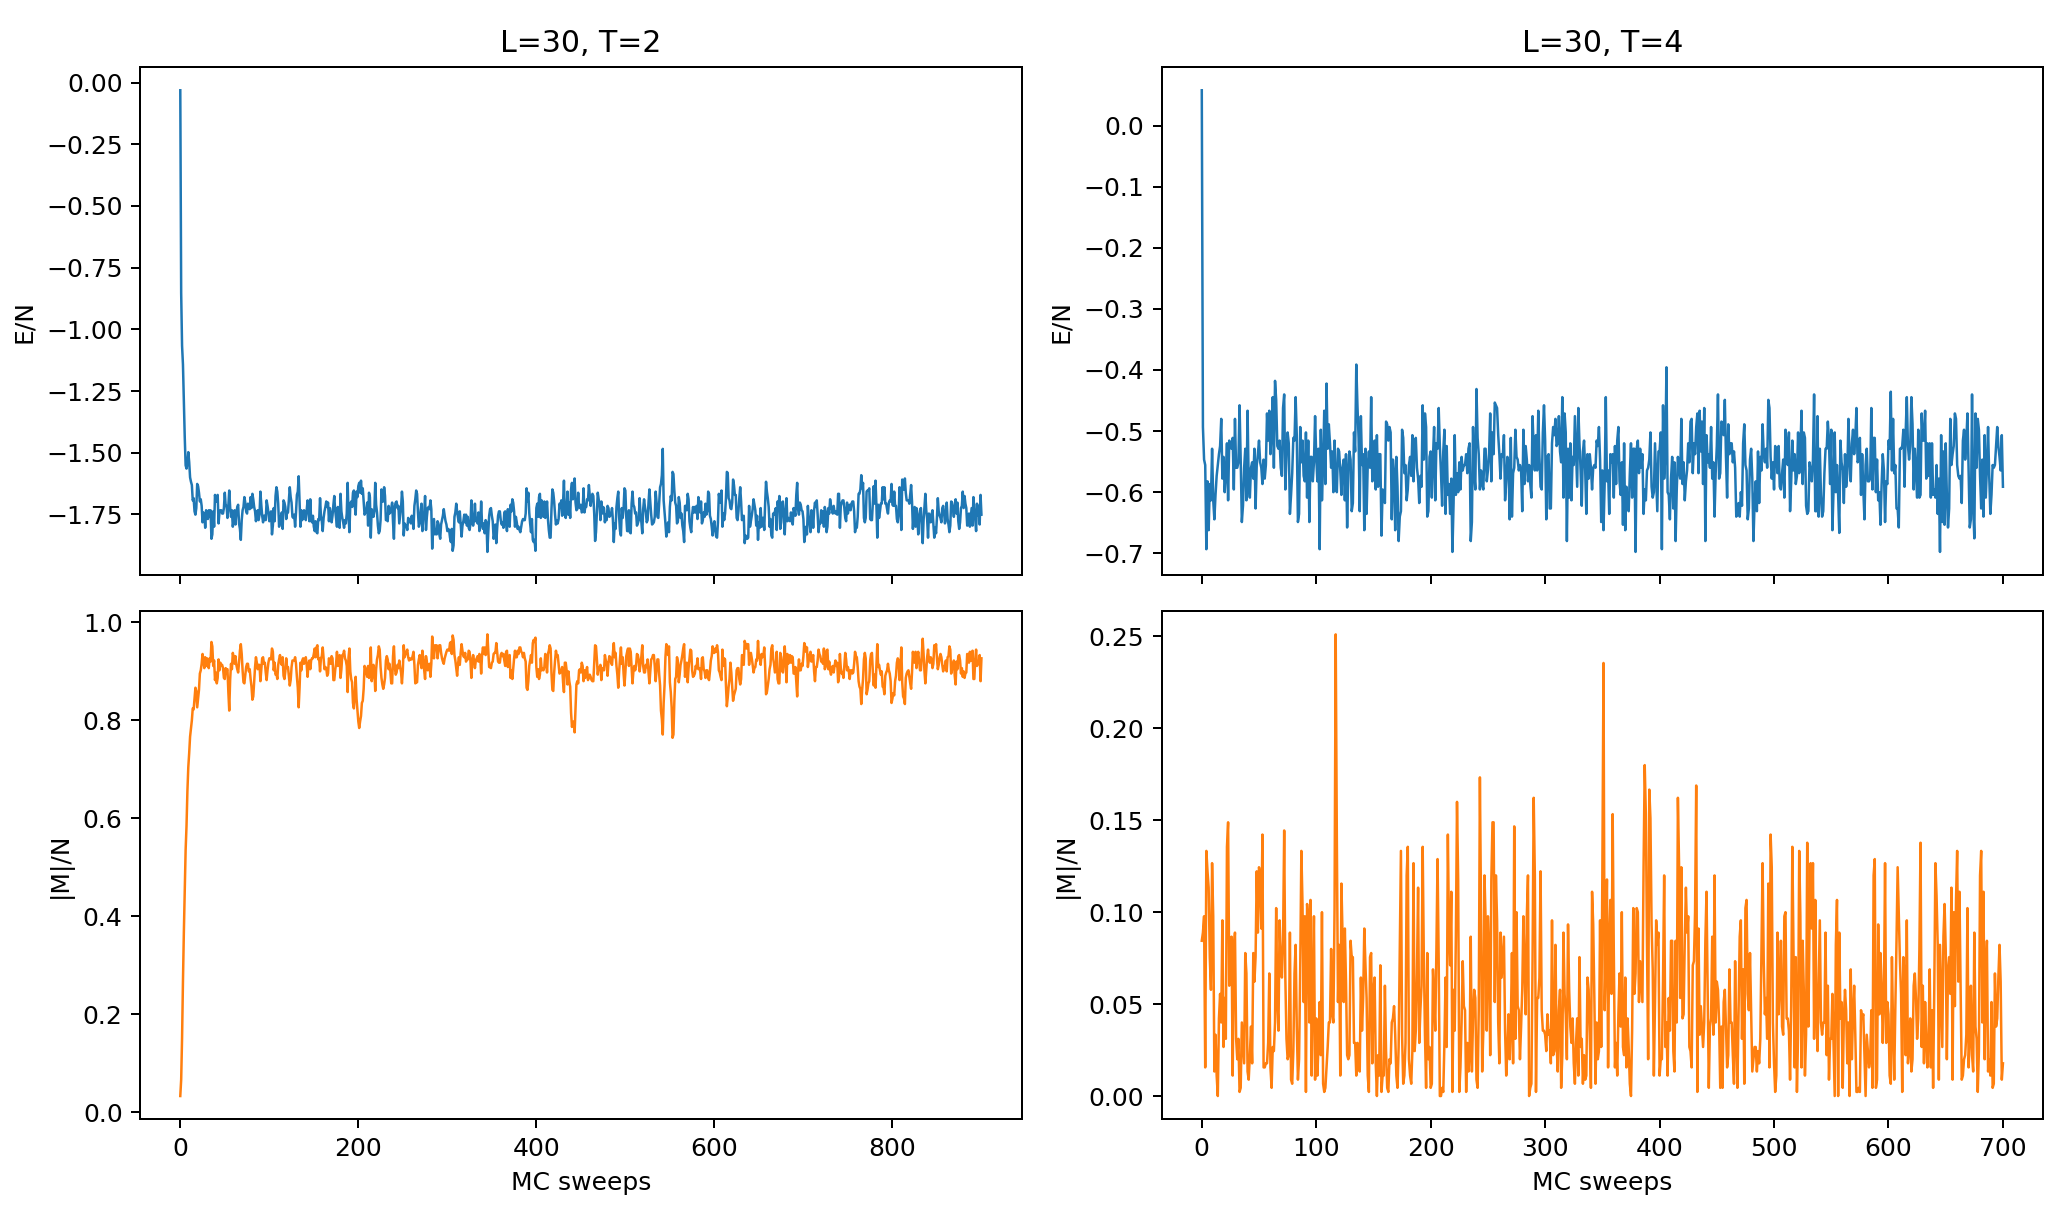
\includegraphics[width=0.88\linewidth]{problem3_T2_T4_trajectories.png}
  \caption{$L=30$ 时 $T=2$ 与 $T=4$ 的能量和磁化轨迹。}
\end{figure}

\begin{figure}[H]
  \centering
  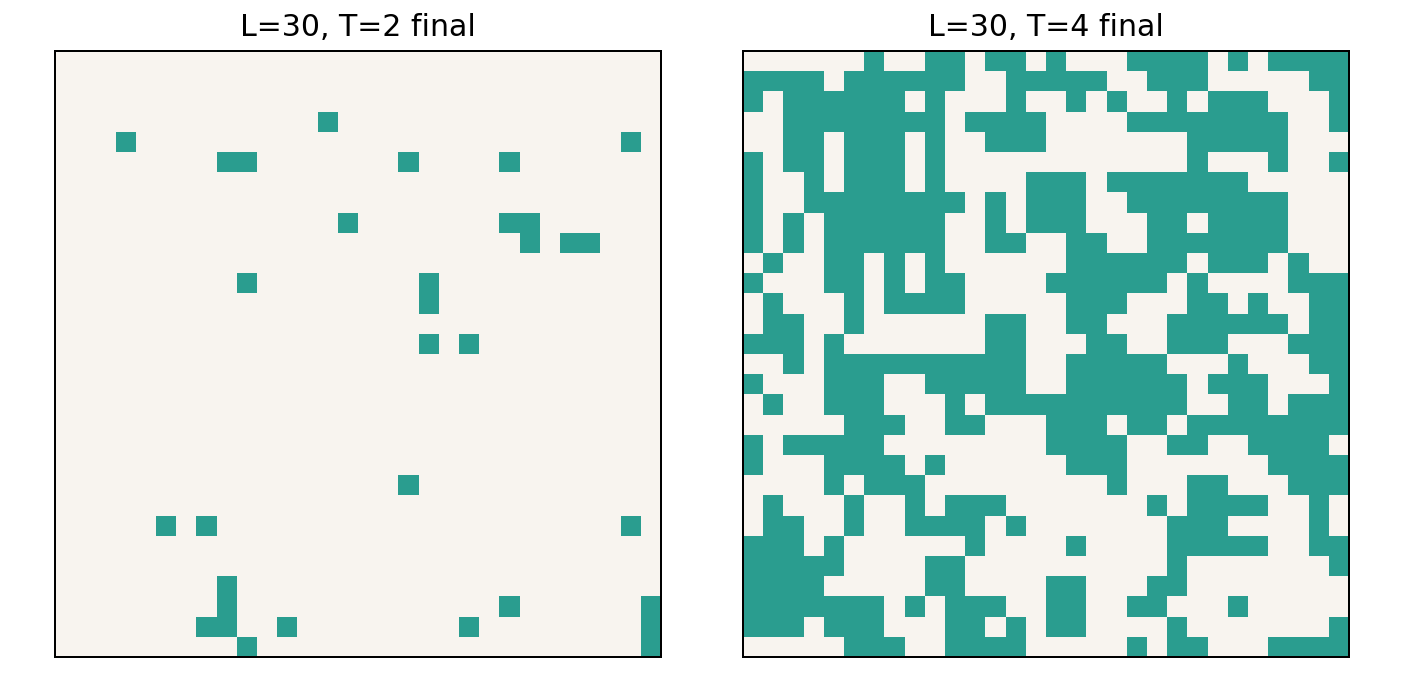
\includegraphics[width=0.62\linewidth]{problem3_T2_T4_snapshots.png}
  \caption{$T=2$ 和 $T=4$ 的最终自旋图样。}
\end{figure}

\blocktitle{理解}
$T=2$ 低于 $T_c\simeq2.269$，畴会并合并形成宏观磁化；$T=4$ 中热涨落破坏长程序，末态保持无序。

\problem{Problem 3(c)--(h)：初态、边界、比热与采样方式}

\blocktitle{待求问题}
改变初态、系统尺寸、边界条件、更新顺序和采样频率，判断平衡统计和弛豫时间如何变化。

\blocktitle{解决方式}
温度扫描中用涨落法和数值微分同时估计比热：
\[
  \frac{C}{N}=\frac{\langle E^2\rangle-\langle E\rangle^2}{NT^2},\qquad
  \frac{C}{N}\simeq\frac{d(E/N)}{dT}.
\]
开放边界只统计实际存在的水平和竖直键；更新顺序比较使用相同的单自旋 Metropolis 接受规则。

\blocktitle{问题答案}
\begin{figure}[H]
  \centering
  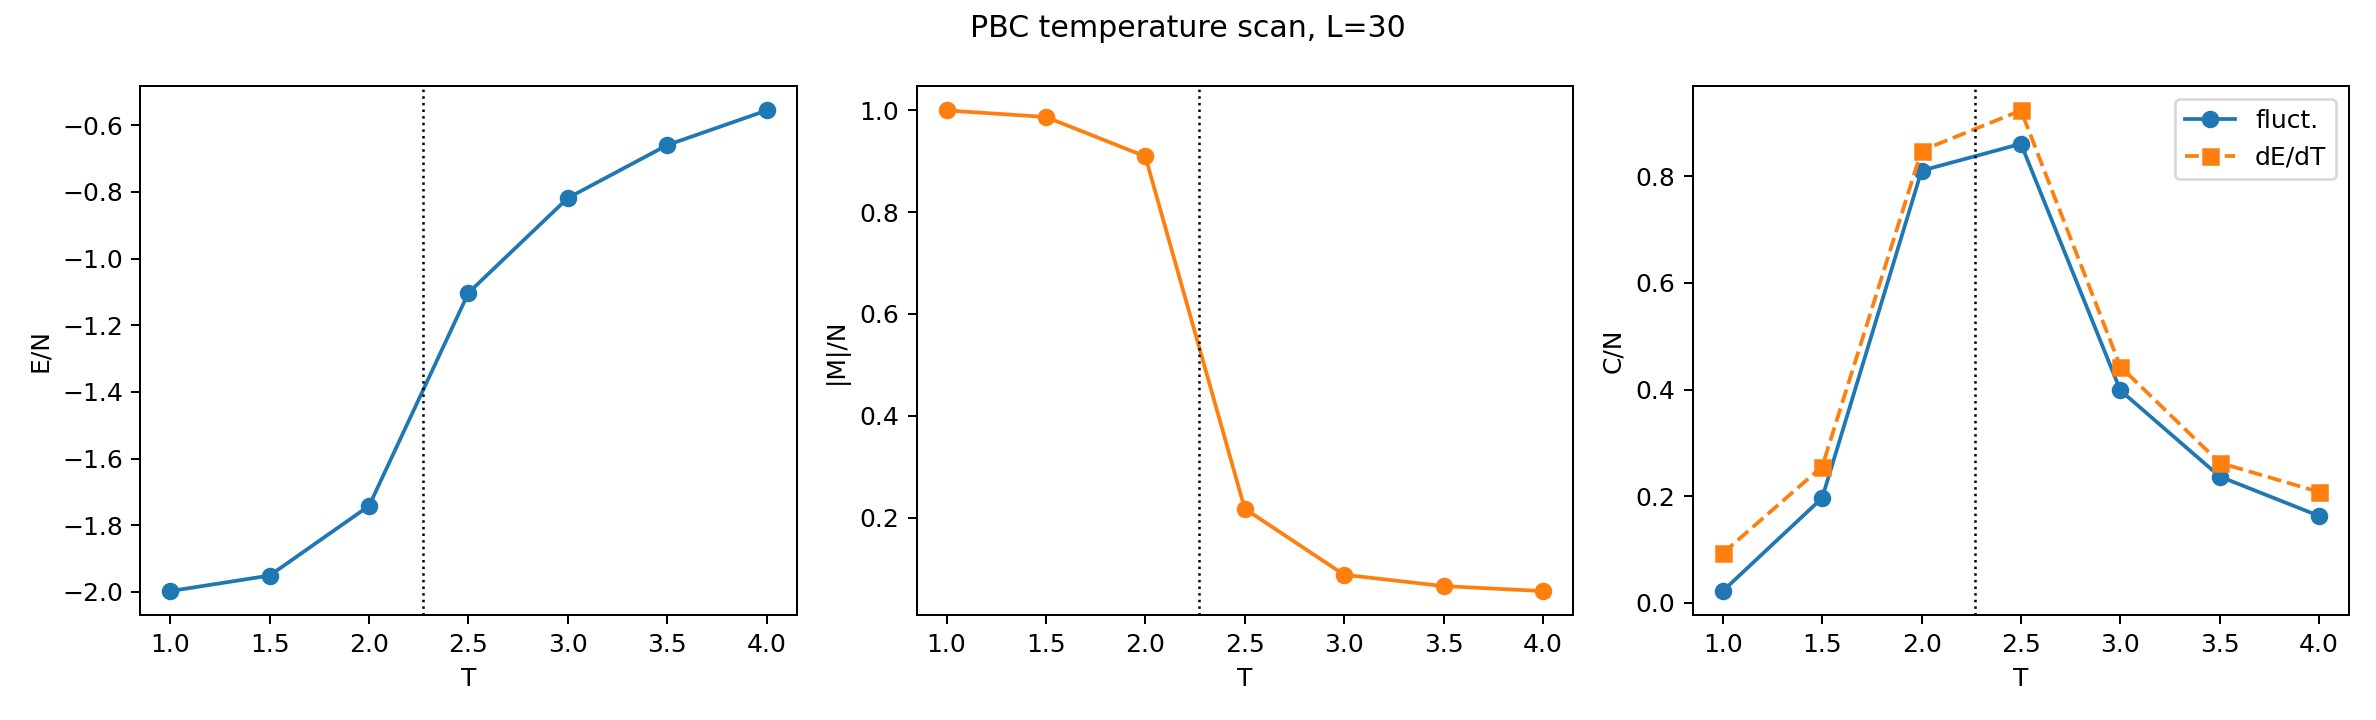
\includegraphics[width=0.92\linewidth]{problem3_L30_temperature_scan.png}
  \caption{$L=30$ 周期边界温度扫描。}
\end{figure}

$L=30$ 的磁化突降和比热峰均出现在 $T=2.0$ 到 $2.5$ 之间，接近二维热力学极限临界温度。开放边界会降低平均配位数，使 $E/N$ 绝对值和 $\langle |m|\rangle$ 降低；这个效应在 $L=4$ 中更强。随机选点与有序扫描的有限时间结果不同，反映了临界附近的强时间相关。

\begin{figure}[H]
  \centering
  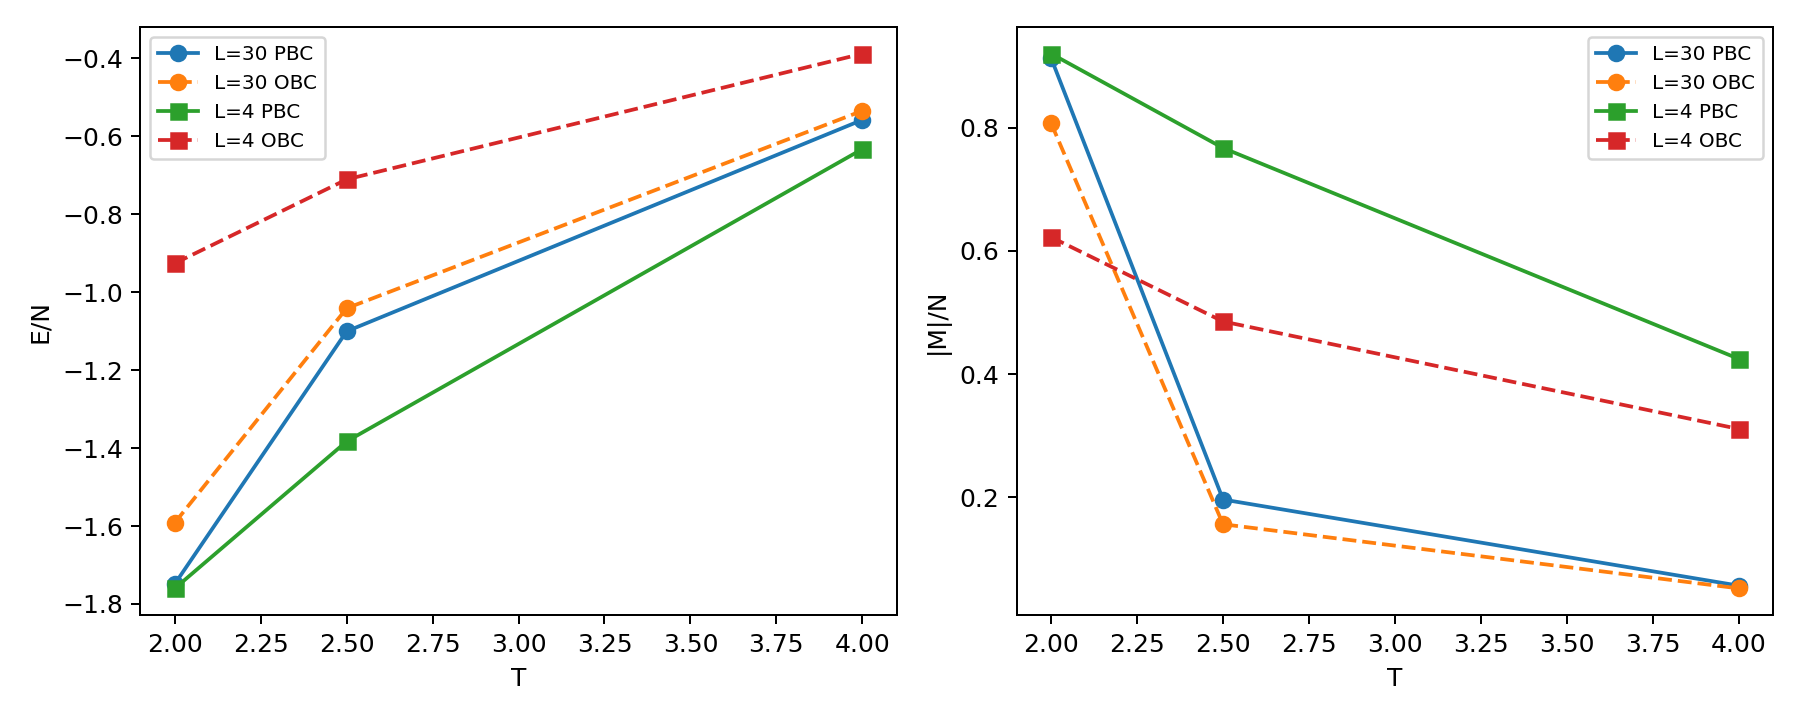
\includegraphics[width=0.82\linewidth]{problem3_obc_comparison.png}
  \caption{开放边界与周期边界比较。}
\end{figure}

\blocktitle{理解}
这些对照说明局域 Metropolis 不只给出平衡分布，也携带明显的算法动力学特征。有限运行时间下，初态、边界和扫描顺序都会影响估计值。

\section*{IV. 二维 Ising 模型磁化与有限尺寸标度}

\problem{Problem 4(a)--(d)：磁化曲线和临界指数}

\blocktitle{待求问题}
用 MCMC 模拟二维 Ising 的磁化随温度变化，并由 $\ln\langle m^2\rangle$ 与 $\ln L$ 的关系估计临界指数。

\blocktitle{解决方式}
对 $L=4,8,16,32$ 扫描温度并统计 $\langle |m|\rangle$ 和 $\langle m^2\rangle$。热力学极限的自发磁化用
\[
  m(T)=\left[1-\sinh^{-4}\left(\frac{2}{T}\right)\right]^{1/8},\qquad T<T_c
\]
作参考。临界点附近拟合
\[
  \ln\langle m^2\rangle=a+b\ln L,\qquad b=-2\beta/\nu.
\]

\blocktitle{问题答案}
\begin{figure}[H]
  \centering
  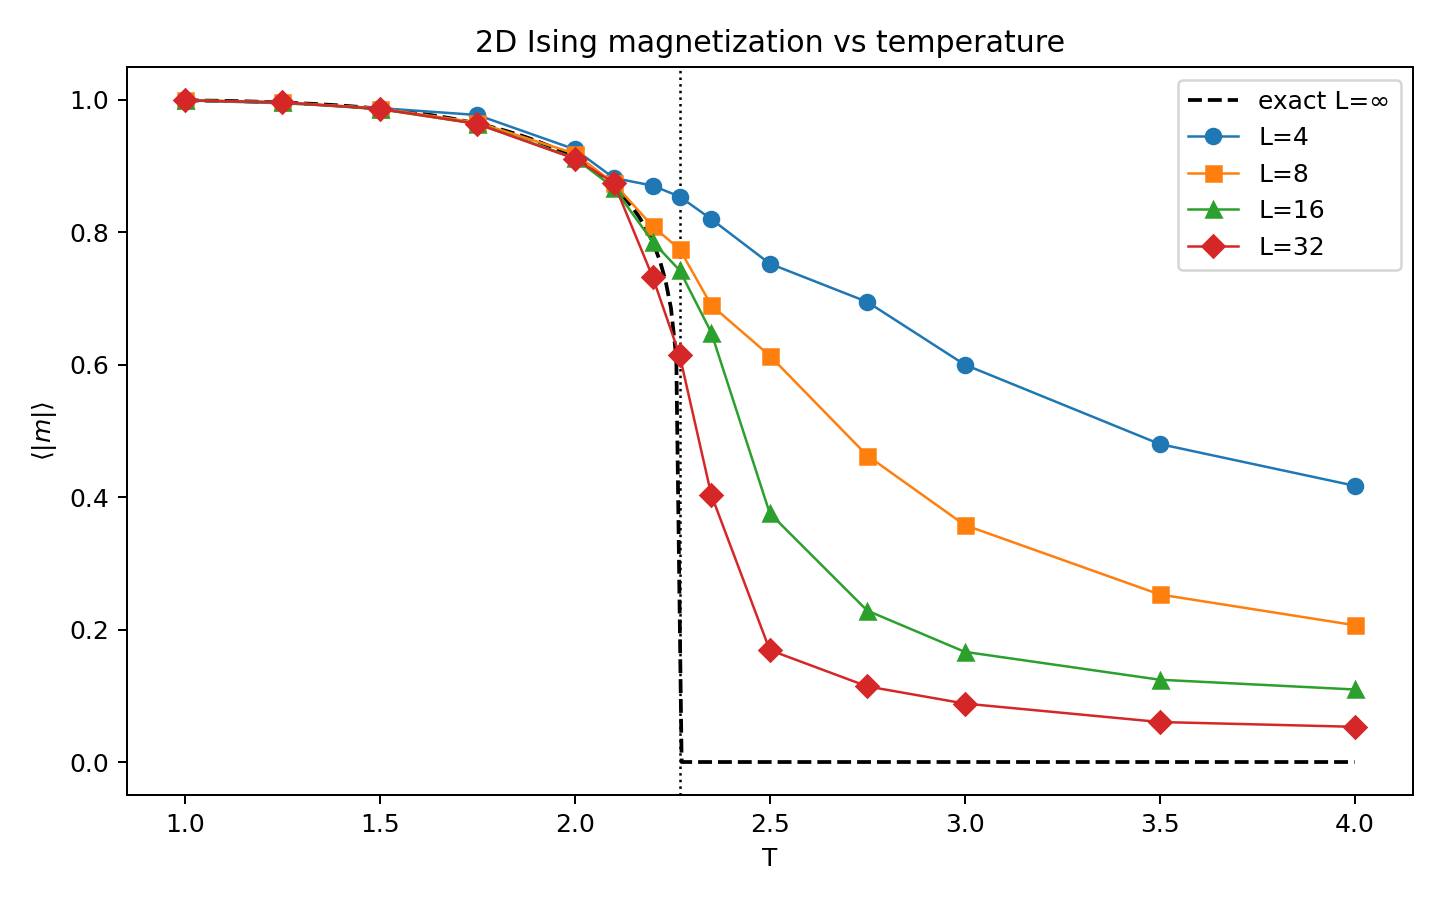
\includegraphics[width=0.82\linewidth]{problem4_magnetization_vs_T.png}
  \caption{不同系统尺寸下的磁化温度曲线。}
\end{figure}

\begin{table}[H]
  \centering
  \caption{有限尺寸标度拟合。}
  \begin{tabular}{rrr}
    \toprule
    $T$ & 斜率 $b$ & $\beta/\nu=-b/2$ \\
    \midrule
    2.000 & -0.026 & 0.013 \\
    2.269 & -0.277 & 0.139 \\
    2.500 & -1.297 & 0.648 \\
    \bottomrule
  \end{tabular}
\end{table}

在 $T=2.269$ 处斜率 $-0.277$ 接近理论值 $-0.25$，得到 $\beta/\nu=0.139$，与理论值 $1/8=0.125$ 接近。

\begin{figure}[H]
  \centering
  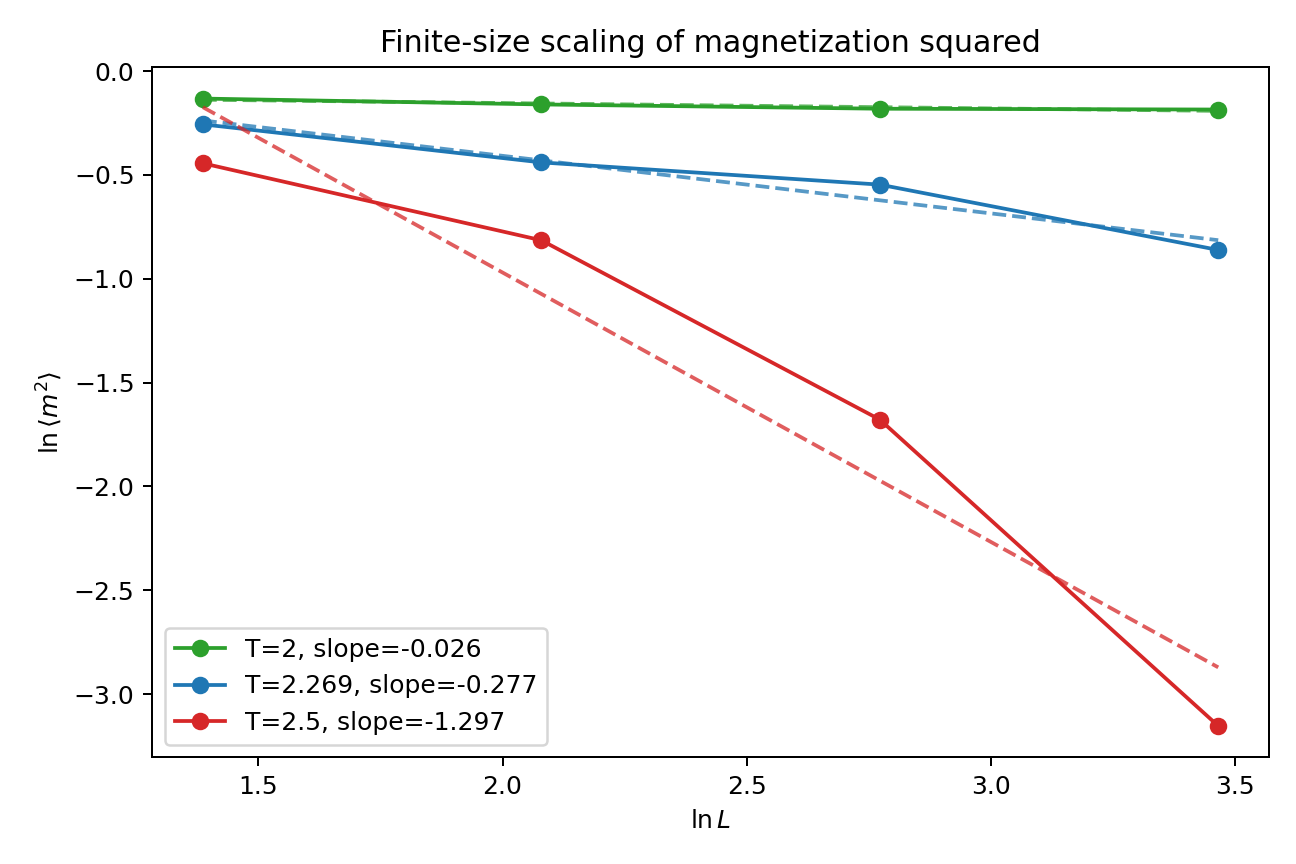
\includegraphics[width=0.74\linewidth]{problem4_fss_logfit.png}
  \caption{$\ln\langle m^2\rangle$ 与 $\ln L$ 的线性拟合。}
\end{figure}

\blocktitle{理解}
只有在临界附近，有限尺寸幂律才直接对应临界指数。低温区 $\langle m^2\rangle$ 几乎不随 $L$ 变化，高温区相关长度有限，斜率也不再是临界指数。

\problem{Problem 4(e)：$100\times100$ 自旋图样}

\blocktitle{待求问题}
展示 $100\times100$ 二维正方格点的 MCMC 图样，并说明 MC sweep 不是物理实时时间。

\blocktitle{解决方式}
从随机初态出发，在 $T=T_c$ 和 $T=2T_c$ 下记录 $t=0,100,200,300$ sweep 的自旋图样。

\blocktitle{问题答案}
\begin{figure}[H]
  \centering
  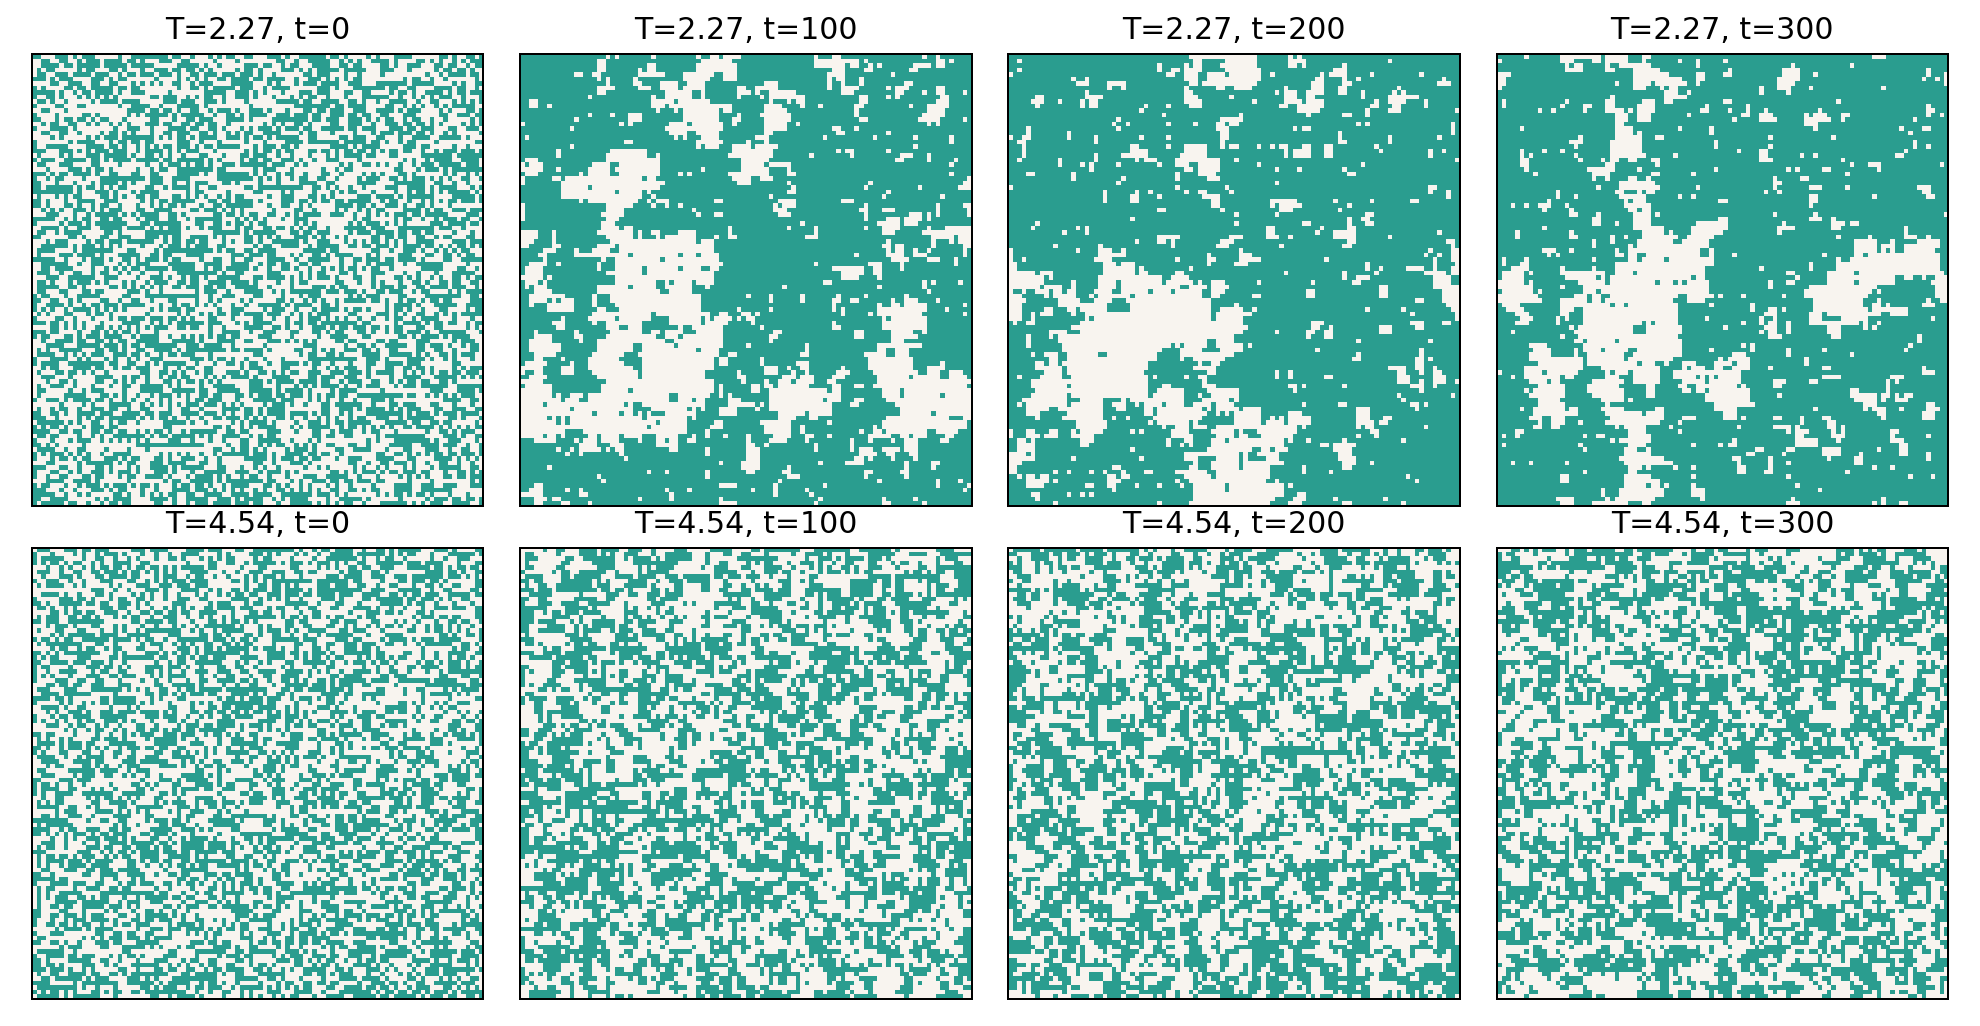
\includegraphics[width=0.92\linewidth]{problem4_L100_snapshots.png}
  \caption{$100\times100$ 二维 Ising 自旋图样演化。}
\end{figure}

\blocktitle{理解}
临界附近出现大尺度团簇，高温下构型保持细碎无序。图样序列反映的是 Markov 链迭代过程，不代表真实动力学时间。

\section*{V. 原生 \LaTeX{} 路线观察}

\plainblocktitle{优势}
原生 \LaTeX{} 对公式、表格、图像位置和算法块的控制更直接。本文中所有图均使用 \verb|figure[H]| 固定在对应位置，算法使用 \verb|algorithm2e|，不需要依赖 Pandoc 对 Markdown 属性的解释。

\plainblocktitle{代价}
源文件更冗长，中文、路径、特殊字符和表格语法都需要更谨慎维护。若还需要 docx，原生 \LaTeX{} 不能像 Markdown/Pandoc 那样自然地产生双格式输出。

\plainblocktitle{建议}
若最终交付只看 PDF，并且报告包含大量公式、伪代码和图表，原生 \LaTeX{} 更稳；若需要快速迭代、自动生成或同时导出 docx，Markdown/Pandoc 仍然更方便。

\end{document}
